\chapter{Iteration 1 (FYP-1 Mid)}
\label{ch:iter1}
\begin{itemize}
    \item FYP 1 Mid: 
    \begin{itemize}
    \item Literature review related Metaverse, and Healthcare
    \item Designed Use-case, System Diagram
    \end{itemize}
\end{itemize}


\section{Literature review related Metaverse, and Healthcare}
{The aof metaversion, a virtual, interconnected digital realm, into the healthcare field represents a promising frontier in medical technology and patient care. As technology continues to advance, metaverse offers innovative solutions to long-standing challenges in the healthcare industry, from medical training and telemedicine to mental health therapy and patient empowerment. This literature review aims to provide a comprehensive examination of current research, technology and developments in the use of metaversion in healthcare. By examining the historical perspective, technological foundations, practical applications, ethical considerations, and future prospects of metaversion in healthcare, this review seeks to illuminate the current state of knowledge and pave the way for further advances in this rapidly evolving field.
}

\section{Designed Use-case, System Diagram}
\begin{itemize}
    \item Use Case 
    \item System Diagram
    \item Activity Diagram
\end{itemize}


\section{Use Case Diagram}
A use case diagram represents the main use case activities and the interaction of actors and the system that is under development process. It helps to identify all main processes of the system which are then visualized in ovals, known as a use case. A use case diagram is drawn from a scenario that explains the working of the system.
\begin{figure}[h]
    \centering
    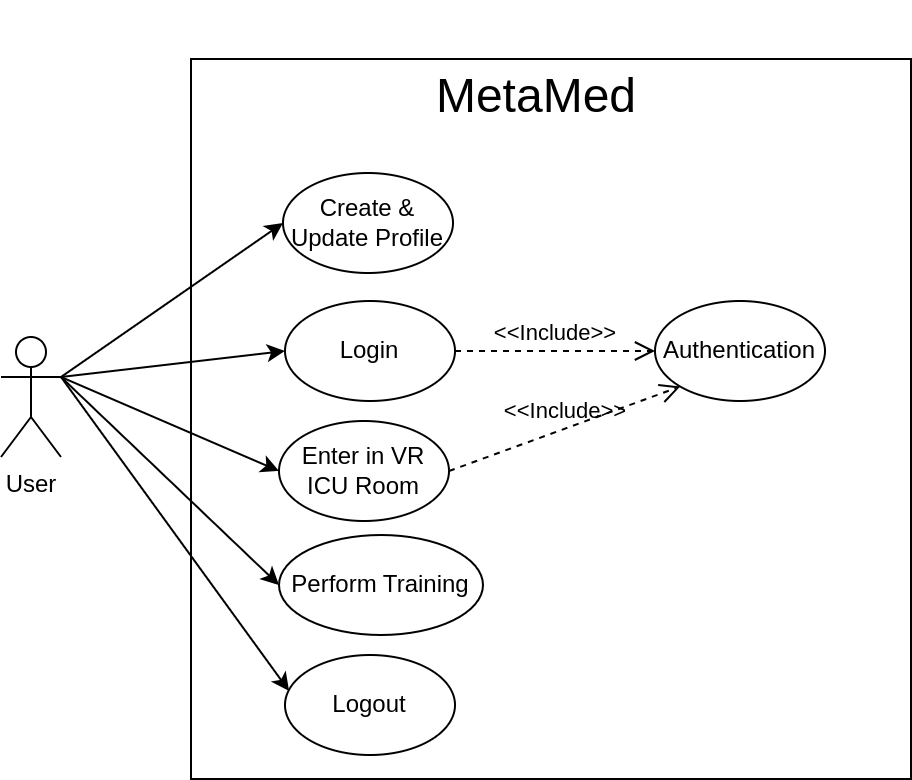
\includegraphics[width=0.5\textwidth, height=0.3\textheight]{Images/Use Case.drawio.png}
    \caption{Use Case Diagram}
    \label{fig:system-diagram}
\end{figure}


\section{System Diagram}
System Diagrams are models used to visually express the dynamic forces acting upon the components of a process and the interactions between those forces. System Diagrams are more than process flow charts.
\begin{figure}[h]
    \centering
    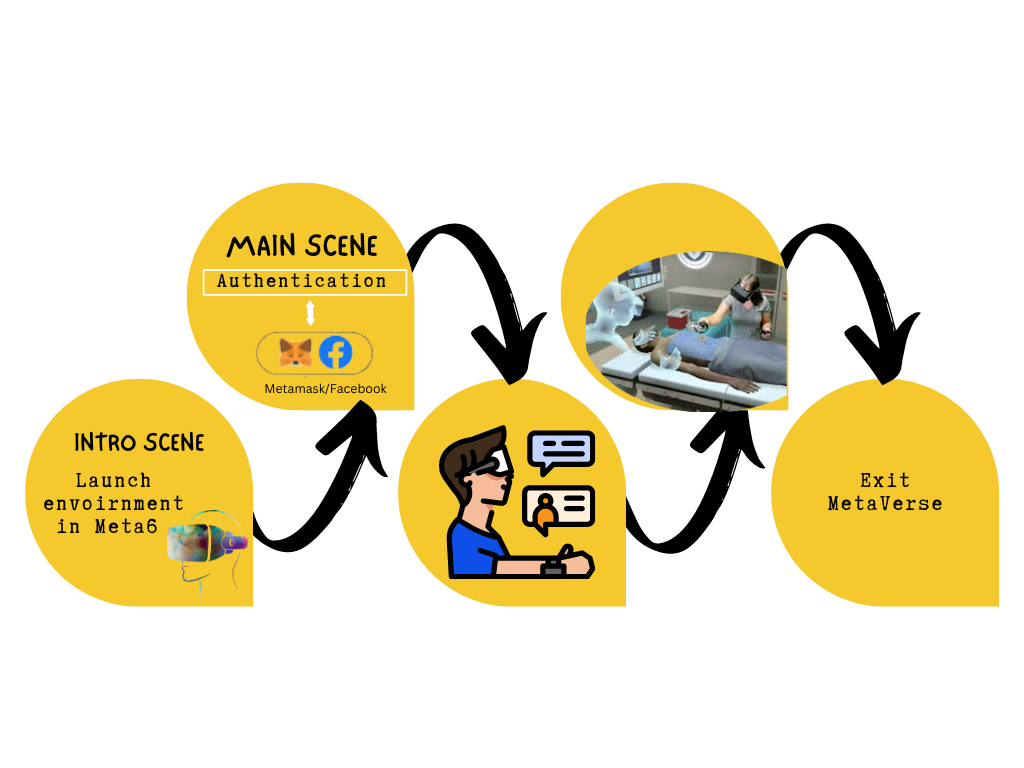
\includegraphics[width=0.7\textwidth, height=0.3\textheight]{Images/system.png}
    \caption{System Diagram}
    \label{fig:system-diagram}
\end{figure}





\section{Activity Diagram}
Activity diagram is a visual representation of a system’s behavior, showing how activities and actions are executed in a particular process or use case. Activity diagrams are used to model a variety of systems and processes, including business workflows, software systems, and organizational processes.
\begin{figure}[h]
    \centering
    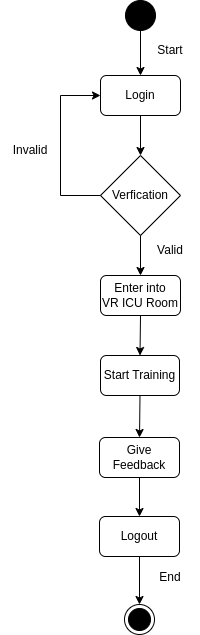
\includegraphics[width=0.3\textwidth, height=0.6\textheight]{Images/Activity.drawio.png}
    \caption{Activity Diagram}
    \label{fig:system-diagram}
\end{figure}